% Prova del 13/02/2023, esercizio 1 (catalogo B70-E01): diffrazione di un urto piano attorno a uno spigolo.
% Numeri e figure: calcoli.py (stessa cartella).

\documentclass[11pt,a4paper]{article}

\usepackage[T1]{fontenc}
\usepackage[utf8]{inputenc}
\usepackage[italian]{babel}
\usepackage{amsmath,amssymb}
\usepackage[a4paper,margin=2.4cm]{geometry}
\usepackage{array}
\usepackage{siunitx}
\usepackage{booktabs}
\usepackage{graphicx}
\usepackage{float}
\usepackage{hyperref}

\hypersetup{hidelinks}
\setlength{\parindent}{0pt}
\setlength{\parskip}{4pt}
\allowdisplaybreaks
\graphicspath{{figure/}}
\sisetup{output-decimal-marker={,}, group-separator={\,}, per-mode=symbol,
         exponent-product=\cdot, range-phrase={\text{--}}}

\newcommand{\Ms}{M_{s}}
\newcommand{\Cp}{C^{+}}

\title{Gasdinamica -- Prova del 13/02/2023, esercizio 1\\[2pt]
\large Diffrazione di un urto piano attorno a uno spigolo}
\author{}
\date{}

\begin{document}
\maketitle

\section*{Traccia}
Un urto piano con numero di Mach $\Ms=4$ si diffrange attorno a uno spigolo vivo C formato da due pareti piane con
angolo di \ang{105} (fotografia schlieren, fig.~\ref{fig:ann}). Il gas indisturbato davanti all'urto è aria a
$p=\SI{1e5}{Pa}$ e $T=\SI{293}{K}$. Il rapporto fra la posizione della testa A (distanza misurata dall'ascissa
dello spigolo C) e quella del piede B (distanza misurata lungo la parete inclinata a partire da C) dell'urto diffratto
DS vale $2{,}5$. La linea di separazione SL, che parte da C, presenta una prima deviazione $\theta_1=\ang{44}$ e una
seconda deviazione $\theta_2=\ang{17}$ nel punto F. Determinare: lo stato dietro l'urto piano prima della
diffrazione; la velocità del piede B dell'urto diffratto; l'intensità dell'espansione di Prandtl--Meyer centrata in C,
giustificandone la presenza e spiegando perché il suo fronte di testa termina in D; l'intensità dell'espansione in F;
l'intensità dell'urto di ricompressione RC, giustificandone presenza e geometria; spiegare la presenza della
discontinuità di contatto CD e perché si estende dal punto E, che si muove lungo la parete inclinata come il piede
dell'urto diffratto, fino a D; tracciare le linee di corrente in tutto il campo; determinare la deviazione della linea di
separazione in C nel campo asintotico.

%==============================================================================
\section{Lettura del testo e dell'immagine}
La schlieren (fig.~\ref{fig:ann}) mostra un'istantanea: l'urto piano, che si muove verso destra lungo la parete
superiore, ha appena superato lo spigolo C. La regione scura in basso a sinistra è il corpo: la parete orizzontale
termina in C e prosegue con la parete inclinata CB. Il campo è \textbf{instazionario}: le strutture si allontanano da C
nel tempo. Le frecce a sinistra indicano la corrente dello stato 2, cioè il gas già investito dall'urto piano. La
tecnica rende visibili i gradienti di densità: gli urti sono linee nette e sottili, il contatto è una linea più
sfumata, le espansioni sono zone d'ombra estese. Non c'è scala delle lunghezze: tutte le distanze sono riferite a
$x_A$, la distanza di A dall'ascissa di C.

Dati: aria, $\gamma=1{,}4$, $R=\SI{287}{J/(kg.K)}$; stato 1 (gas fermo) $p_1=\SI{1e5}{Pa}$, $T_1=\SI{293}{K}$;
$\Ms=4$; $x_A/s_B=2{,}5$; $\theta_1=\ang{44}$, $\theta_2=\ang{17}$; deviazione della parete in C pari a \ang{105}.
Interpreto ``corner angle'' come la rotazione della parete rispetto alla corrente: la parete inclinata forma
\ang{105} con il verso della corrente 2, cioè \ang{75} con la parete orizzontale (lo conferma la misura, §4).

%==============================================================================
\section{Identificazione delle strutture}
\begin{itemize}
\item \textbf{AD}: tratto ancora rettilineo e verticale dell'urto incidente, mobile verso destra con
  $W=\Ms a_1$. Lassù non è ancora arrivata alcuna informazione dallo spigolo.
\item \textbf{DS}: urto diffratto, curvo, dal punto D fino al piede B sulla parete inclinata. È una linea netta, quindi
  un urto. Si indebolisce da D (intensità dell'urto piano) a B, e in B arriva ortogonale alla parete.
\item \textbf{Ventaglio in C}: zona scura che parte da C e si apre verso destra. È l'espansione di Prandtl--Meyer
  con cui la corrente 2 gira attorno allo spigolo; a una parete sotto la corrente che ruota verso il basso corrisponde
  un'onda $\Cp$.
\item \textbf{SL}: linea di separazione (strato di scorrimento) che si stacca dallo spigolo. La corrente non segue la
  parete e se ne separa. Sotto SL c'è una bolla di ricircolo; in fondo a SL lo strato si avvolge in un vortice (la zona
  scura e sfumata vicino all'estremo inferiore di SL).
\item \textbf{F}: spigolo di SL, dove la corrente ruota di altri \ang{17}. È il centro di una seconda espansione $\Cp$.
\item \textbf{RC}: urto di ricompressione, la linea luminosa netta più interna. Parte dall'estremo di SL e risale
  curvandosi; verso l'alto diventa sfumata e scompare dentro il ventaglio.
\item \textbf{CD}: discontinuità di contatto, la linea intermedia fra RC e DS, meno netta di DS. Va da D (dove si
  avvicina a DS) fino alla parete inclinata in E, passando sotto il vortice.
\end{itemize}
Il cerchio chiaro nel corpo è un dettaglio dell'apparato (oblò o presa), estraneo al campo. Le linee sottili
verticale e orizzontale per C e i segmenti indicati con $\theta_1$, $\theta_2$ sono riferimenti disegnati sulla traccia.

\begin{figure}[H]
  \centering
  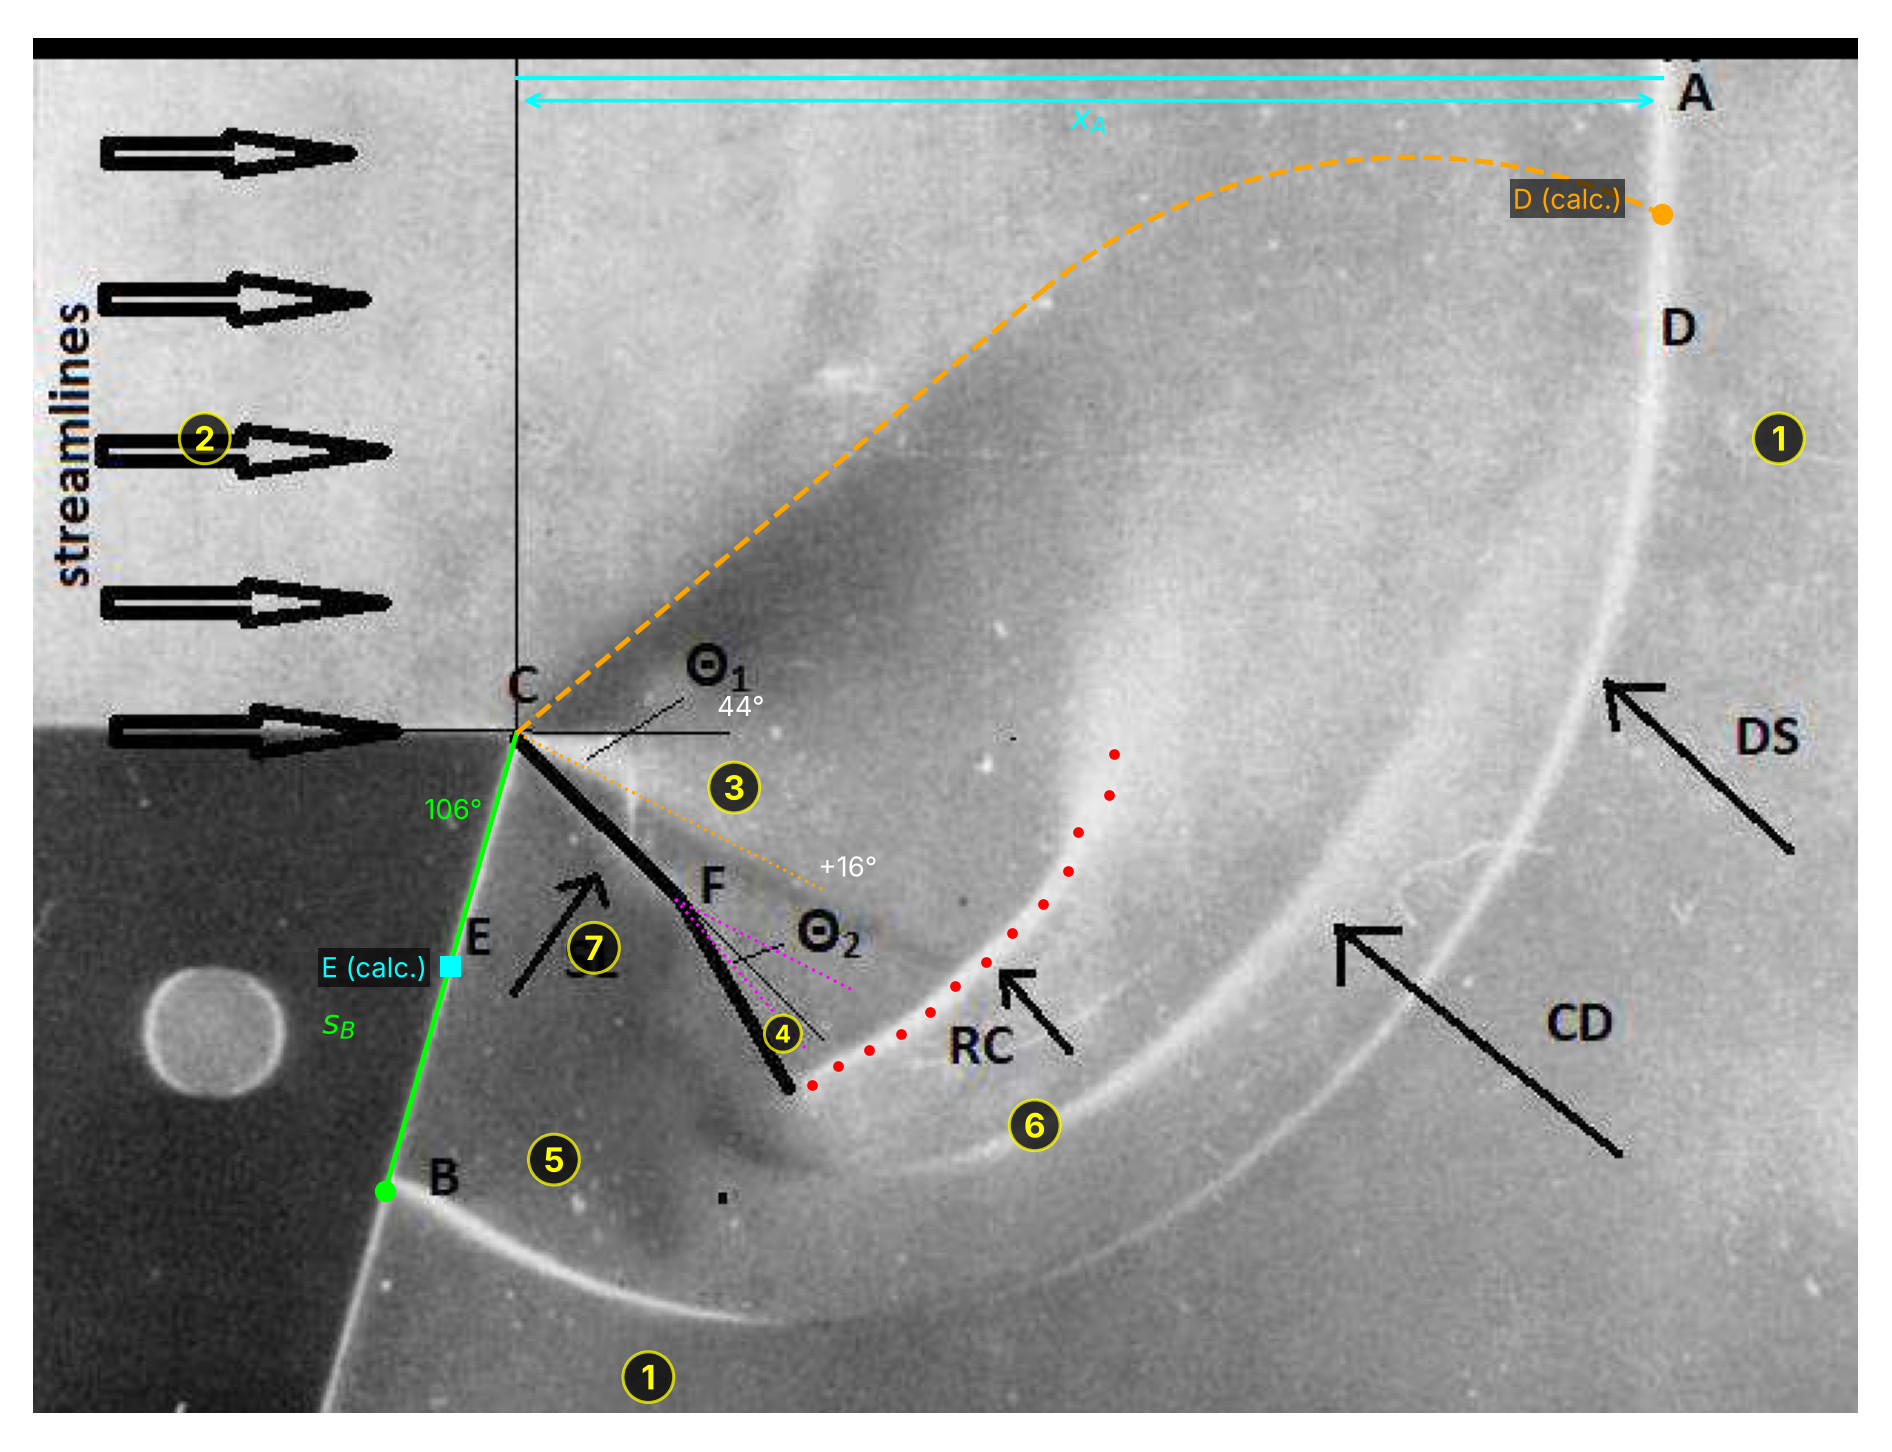
\includegraphics[width=0.92\textwidth]{annotata.png}
  \caption{Schlieren della traccia con le strutture e le misure. Verde: parete inclinata CB (deviazione misurata
  \ang{106}); azzurro: $x_A$ e posizione calcolata di E; arancio tratteggiato: testa del ventaglio di C calcolata
  (retta di Mach da C fino a T, poi arco del cerchio acustico fino a D); arancio puntinato: coda del ventaglio di C;
  magenta: testa e coda del ventaglio in F; punti rossi: RC misurato. I numeri indicano gli stati.}
  \label{fig:ann}
\end{figure}

%==============================================================================
\section{Ipotesi e modello}
\begin{enumerate}
\item \textbf{Gas perfetto, non viscoso fuori da SL.} Aria con $\gamma=1{,}4$. La viscosità conta solo nello strato
  di scorrimento SL e nella bolla di ricircolo, che tratto come un contorno: SL è un contorno libero, attraverso cui
  pressione e direzione della velocità sono continue.
\item \textbf{Campo piano e autosimile.} Le pareti sono piane e lo spigolo è l'unico punto singolare: senza una
  lunghezza di riferimento, il campo dipende solo da $x/t$ e $y/t$ (pseudo-stazionario). Ogni punto della
  configurazione si allontana da C con velocità proporzionale alla sua distanza da C. Ne discende che
  $x_A/s_B$ è anche il rapporto fra le velocità di A e di B. L'immagine lo conferma: le strutture sono
  geometricamente simili a sé stesse e convergono tutte in C.
\item \textbf{Corrente 2 uniforme e stazionaria} prima di essere raggiunta dai disturbi di C: il gas è investito da un
  urto piano a $\Ms$ costante.
\item \textbf{Intorno di C stazionario.} Vicino a C la corrente vede un contorno fisso (lo spigolo) e una corrente 2
  uniforme e supersonica. Il disturbo dello spigolo resta confinato dietro la sua testa, mentre l'urto si allontana:
  in quella zona la corrente è stazionaria nel riferimento del laboratorio e si usa la teoria 2D supersonica
  stazionaria (onde semplici di Prandtl--Meyer). Va verificato che le regioni interessate siano supersoniche (§8).
\item \textbf{Piede B.} In B l'urto arriva ortogonale alla parete (si vede nell'immagine): localmente è un urto
  normale mobile che investe il gas fermo 1. Per RC, invece, uso la velocità di traslazione stimata con
  l'autosimilarità (§4) e lo tratto come localmente normale alla corrente.
\end{enumerate}
Le zone a valle di DS e di RC e i ventagli non sono uniformi: calcolo gli stati uniformi e, per le zone non uniformi,
solo i valori nei punti significativi.

%==============================================================================
\section{Misure sull'immagine}
Con goniometro e righello sulla fig.~\ref{fig:ann}:
\begin{itemize}
\item parete inclinata: \ang{16} dalla verticale, cioè una deviazione di \ang{106} rispetto alla corrente
  (dato \ang{105});
\item $x_A \approx 400$ unità, $s_B=\overline{CB}\approx 166$ unità, quindi $x_A/s_B\approx 2{,}4$ (dato $2{,}5$);
\item SL: primo tratto a \ang{44} sotto l'orizzontale, secondo a \ang{60}, quindi $\theta_2\approx\ang{16}$
  (dati \ang{44} e \ang{17});
\item bordo superiore della zona scura uscente da C: circa \ang{43} sopra l'orizzontale;
\item il tratto rettilineo AD finisce, a occhio, a circa $0{,}35\,x_A$ sopra C (D è dove DS comincia a curvarsi);
\item RC: il tratto inferiore dista da C circa quanto B, da $0{,}96\,s_B$ a $1{,}06\,s_B$; la sua normale è
  inclinata di circa \ang{58} sotto l'orizzontale, quasi parallela alle correnti 3 e 4. La velocità normale di RC è
  quindi $\approx 0{,}95\,W_B$: nel seguito assumo $W_{RC}\approx W_B$, diretta come la corrente.
\end{itemize}
Le misure confermano i dati della traccia; nel calcolo uso i valori assegnati.

%==============================================================================
\section{Analisi qualitativa e topologia}
\textbf{Prima della diffrazione.} Il gas fermo 1 attraversa l'urto piano (onda $u+a$, che spinge il gas nel verso in cui
si propaga) e passa nello stato 2. Con $\Ms=4$ la corrente 2 è \textbf{supersonica nel riferimento del
laboratorio} ($M_2>1$ per $\Ms>2{,}07$). Quando l'urto supera C, la corrente 2 trova la parete che si ritira e deve
girare attorno allo spigolo. Essendo supersonica, gira con un \textbf{ventaglio di Prandtl--Meyer centrato in C}.
Con $M_2<1$ non ci sarebbe un ventaglio centrato, ma un'accelerazione subsonica attorno allo spigolo.

\textbf{Testa del ventaglio e punto D.} I disturbi emessi da C quando l'urto vi passa ($t=0$) si propagano con la
velocità del suono $a_2$ rispetto al gas, che si muove con $u_2$. All'istante $t$ occupano il cerchio di centro
$(u_2t,0)$ e raggio $a_2t$. Nella parte vicina a C l'inviluppo di questi cerchi è la retta di Mach uscente da C a
$\mu_2$ sulla corrente (tratto stazionario), tangente al cerchio in T; oltre T il fronte è l'arco del cerchio stesso.
L'urto piano è subsonico rispetto al gas che ha dietro ($W-u_2<a_2$): il cerchio lo raggiunge, e lì nasce D. Oltre
l'urto il disturbo non passa, perché davanti c'è il gas 1 fermo e l'urto è supersonico rispetto a esso. Per questo
la testa termina in D, e sopra D l'urto resta piano.

\textbf{Urto diffratto.} Sotto D l'urto, ``alimentato'' da un gas che si espande, si indebolisce e si curva fino a
raggiungere la parete inclinata in B con intensità molto minore, ortogonale alla parete.

\textbf{Separazione e seconda espansione.} Per seguire la parete la corrente dovrebbe ruotare di \ang{105}: con
$\nu(M_2)+\ang{105}$ si arriverebbe praticamente al vuoto (§7c). Lo strato limite si separa nello spigolo e la corrente
si espande solo fino alla pressione della bolla di ricircolo sotto SL, ruotando di $\theta_1$. Più a valle lo strato
separato si avvolge nel vortice, il cui nucleo è a pressione più bassa. Per questo SL piega di nuovo in F e la corrente
si espande ancora (ventaglio $\Cp$ centrato in F).

\textbf{Ricompressione.} Dopo F la corrente 4 è molto veloce e a pressione molto bassa, mentre il gas a valle,
compresso da DS, è a pressione più alta. Il raccordo avviene con un urto: RC.

\textbf{Contatto.} Il gas a sinistra di CD ha attraversato l'urto piano, il più forte, e in parte anche RC. Il gas fra
CD e DS ha attraversato soltanto l'urto diffratto, più debole. Le due masse hanno entropie diverse e si toccano a
pressione e velocità normale uguali: c'è una discontinuità di contatto.

\textbf{Stati} (fig.~\ref{fig:ann}): 1 gas fermo; 2 dietro l'urto piano; 3 fra la coda del ventaglio di C e la
testa del ventaglio in F; 4 dopo il ventaglio in F, lungo il secondo tratto di SL; 5 dietro il piede B; 6 dietro RC
(non uniforme); 7 bolla di separazione sotto SL vicino a C, che coincide con lo stato asintotico. Il ventaglio di C e
la zona fra CD e DS non sono uniformi.

\begin{figure}[H]
  \centering
  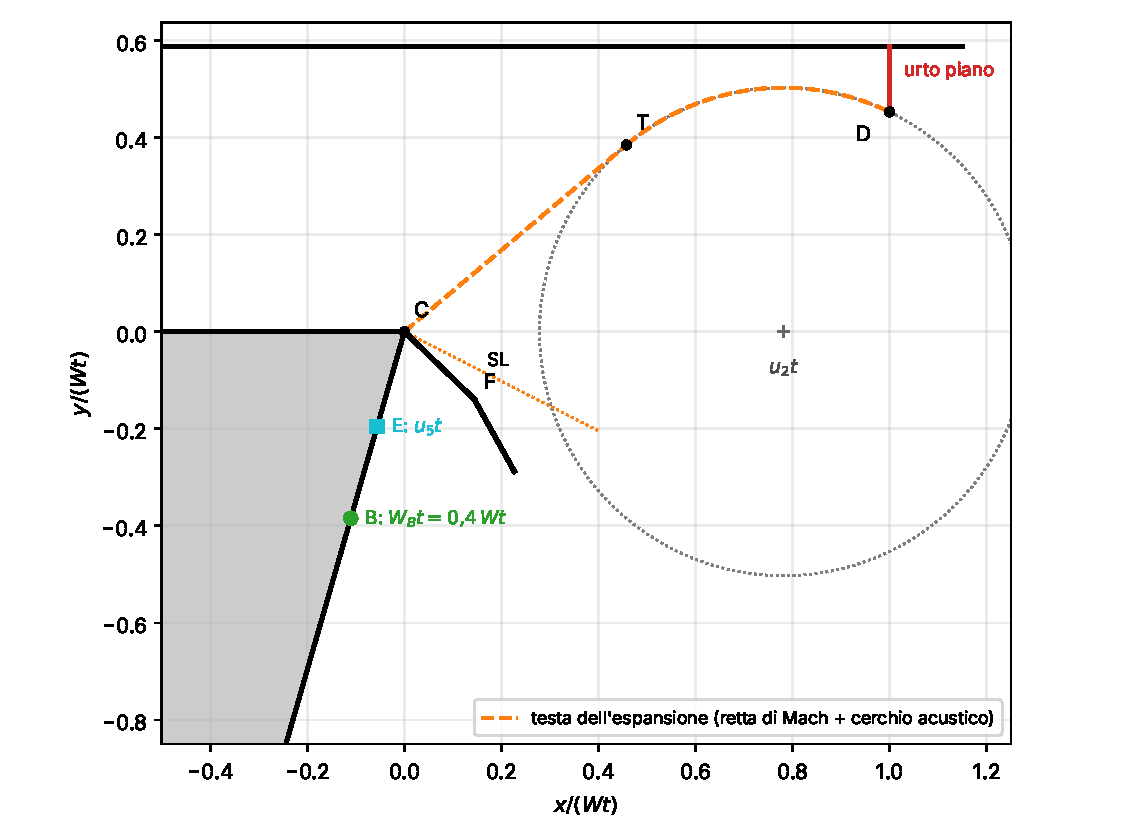
\includegraphics[width=0.66\textwidth]{schema.pdf}
  \caption{Costruzione autosimile (lunghezze divise per $Wt$, origine in C): urto piano in $x=Wt$, cerchio acustico
  emesso da C a $t=0$ (centro $u_2t$, raggio $a_2t$), retta di Mach da C tangente in T, punto D; piede B
  ($W_Bt=0{,}4\,Wt$) e punto E ($u_5t$) sulla parete; SL con lo spigolo F e coda del ventaglio di C.}
  \label{fig:schema}
\end{figure}

%==============================================================================
\section{Calcolo}

\subsection*{a) Stato 1 e urto piano: stato 2}
\[
a_1=\sqrt{\gamma R T_1}=\sqrt{1{,}4\cdot287\cdot293}=\SI{343}{m/s},\qquad W=\Ms a_1=4\cdot343=\SI{1372}{m/s}.
\]
Relazioni di Rankine--Hugoniot nel riferimento dell'urto ($M_{r1}=\Ms=4$):
\[
\frac{p_2}{p_1}=\frac{2\gamma\Ms^2-(\gamma-1)}{\gamma+1}=\frac{2{,}8\cdot16-0{,}4}{2{,}4}=18{,}5,
\]
\[
\frac{\rho_2}{\rho_1}=\frac{(\gamma+1)\Ms^2}{(\gamma-1)\Ms^2+2}=\frac{2{,}4\cdot16}{0{,}4\cdot16+2}=4{,}571,
\]
\[
\frac{T_2}{T_1}=\frac{18{,}5}{4{,}571}=4{,}047\ \Rightarrow\ T_2=\SI{1186}{K},\quad
a_2=a_1\sqrt{4{,}047}=\SI{690}{m/s}.
\]
Dalla continuità $\rho_1W=\rho_2(W-u_2)$:
\[
u_2=W\left(1-\frac{\rho_1}{\rho_2}\right)=1372\,(1-0{,}2188)=\SI{1072}{m/s},
\]
\[
M_2=\frac{u_2}{a_2}=\frac{1072}{690}=1{,}55,\qquad p_2=\SI{18.5e5}{Pa}.
\]
La corrente 2 è supersonica. La pressione totale vale
$p_{02}=p_2(1+\delta M_2^2)^{\gamma/(\gamma-1)}=18{,}5\cdot1{,}483^{3{,}5}\cdot10^5=\SI{73.4e5}{Pa}$.

\subsection*{b) Piede B: velocità e stato 5}
Per l'autosimilarità A e B si allontanano da C con velocità proporzionali alle distanze. A appartiene al tratto
piano, che si muove con $W$:
\[
W_B=\frac{s_B}{x_A}\,W=\frac{1372}{2{,}5}=\SI{549}{m/s},\qquad M_{sB}=\frac{W_B}{a_1}=\frac{549}{343}=1{,}60.
\]
In B l'urto è normale alla parete e investe il gas fermo 1:
\[
\frac{p_5}{p_1}=\frac{2{,}8\cdot1{,}6^2-0{,}4}{2{,}4}=2{,}82,\qquad
\frac{\rho_5}{\rho_1}=\frac{2{,}4\cdot1{,}6^2}{0{,}4\cdot1{,}6^2+2}=2{,}03,
\]
\[
\frac{T_5}{T_1}=\frac{2{,}82}{2{,}03}=1{,}39,\quad
\]
\[
u_5=W_B\left(1-\frac{\rho_1}{\rho_5}\right)=549\cdot0{,}508=\SI{279}{m/s},
\]
\[
a_5=343\sqrt{1{,}39}=\SI{404}{m/s},\qquad M_5=\frac{279}{404}=0{,}69,\qquad p_5=\SI{2.82e5}{Pa}.
\]
Dietro il piede il gas scorre lungo la parete, verso B, in regime subsonico.

\subsection*{c) Espansione centrata in C: stato 3}
Onda semplice $\Cp$, con $\theta+\nu$ costante e $\theta$ che passa da 0 a $-\theta_1$:
\[
\nu(M_3)=\nu(M_2)+\theta_1=\ang{13.5}+\ang{44}=\ang{57.5}\ \Rightarrow\ M_3=3{,}43.
\]
Il ventaglio è isentropico ($p_{03}=p_{02}$):
\[
p_3=p_2\,\frac{(1+\delta M_2^2)^{3{,}5}}{(1+\delta M_3^2)^{3{,}5}}
=18{,}5\cdot10^5\,\frac{1{,}483^{3{,}5}}{3{,}360^{3{,}5}}=\SI{1.06e5}{Pa},\qquad
\frac{p_3}{p_2}=0{,}057.
\]
Inoltre $a_3=a_2\sqrt{(1+\delta M_2^2)/(1+\delta M_3^2)}=\SI{459}{m/s}$ e $V_3=M_3a_3=\SI{1575}{m/s}$.
Testa del ventaglio: $\mu_2=\arcsin(1/1{,}55)=\ang{40.1}$ sopra l'orizzontale. Coda:
$-\theta_1+\mu_3=-\ang{44}+\ang{16.9}=\ang{-27.1}$.

Notevole: $p_3\approx p_1$. La bolla di separazione vicino allo spigolo è alla pressione del gas indisturbato.

Fronte di testa e punto D (autosimilarità, lunghezze in unità $Wt$): il cerchio acustico ha centro
$u_2/W=0{,}781$ e raggio $a_2/W=0{,}503$; poiché $W-u_2=\SI{300}{m/s}<a_2$ raggiunge l'urto piano a quota
\[
\frac{y_D}{x_A}=\frac{\sqrt{a_2^2-(W-u_2)^2}}{W}=\frac{\sqrt{690^2-300^2}}{1372}=0{,}45 .
\]
La retta di Mach da C lo tocca in T, a distanza $\sqrt{u_2^2-a_2^2}\,t=0{,}60\,Wt$ da C.

Parete attaccata, solo per confronto: $\nu=\ang{13.5}+\ang{105}=\ang{118.5}<\nu_{\max}=\ang{130.4}$, quindi
$M\approx24$ e $p\approx\SI{0.5}{Pa}$. Sarebbe praticamente il vuoto, una situazione fisicamente impossibile: ecco
perché la corrente si separa.

\subsection*{d) Espansione centrata in F: stato 4}
Seconda onda $\Cp$, con $\theta$ che passa da $-\ang{44}$ a $-\ang{61}$:
\[
\nu(M_4)=\ang{57.5}+\ang{17}=\ang{74.5}\ \Rightarrow\ M_4=4{,}75,
\]
\[
p_4=p_2\,\frac{1{,}483^{3{,}5}}{(1+0{,}2\cdot4{,}75^2)^{3{,}5}}=\SI{0.187e5}{Pa},\qquad \frac{p_4}{p_3}=0{,}18 .
\]
Inoltre $a_4=\SI{358}{m/s}$ e $V_4=\SI{1700}{m/s}$. La testa del ventaglio in F è a $\ang{-27.1}$, parallela alla coda
di quello di C: la zona 3 è una striscia uniforme. La coda è a $-\ang{61}+\mu_4=-\ang{61}+\ang{12.2}=\ang{-48.8}$.

\subsection*{e) Urto di ricompressione RC: stato 6}
RC trasla con $W_{RC}\approx W_B\approx\SI{550}{m/s}$ nel verso della corrente (§4) ed è circa normale alle
correnti 3 e 4. Nel suo riferimento il gas lo attraversa con il Mach relativo $M_r=(V-W_{RC})/a$:
\[
\text{corrente 3:}\quad M_r=\frac{1575-549}{459}=2{,}24,\quad \frac{p_6}{p_3}=\frac{2{,}8\cdot2{,}24^2-0{,}4}{2{,}4}=5{,}7
\ \Rightarrow\ p_6\approx\SI{6.0e5}{Pa};
\]
\[
\text{corrente 4:}\quad M_r=\frac{1700-549}{358}=3{,}22,\quad \frac{p_6}{p_4}=11{,}9
\ \Rightarrow\ p_6\approx\SI{2.2e5}{Pa}.
\]
RC non è uniforme: è più intenso dove riceve la corrente 4. Dietro RC il gas è subsonico rispetto all'urto
($M_{r6}=0{,}54$ e $0{,}46$). Salendo nel ventaglio di C la corrente è meno espansa e $M_r$ diminuisce; RC si annulla
dove $(V-W_{RC})/a=1$. Con $V=Ma$ e $a=a_{02}/\sqrt{1+\delta M^2}$ ($a_{02}=\SI{840}{m/s}$) si trova $M=1{,}85$, cioè
$\nu=\ang{22.1}$, $\theta=\ang{-8.6}$: è il raggio del ventaglio inclinato di $\theta+\mu=\ang{24}$ sopra l'orizzontale.
Oltre quel raggio RC degenera in un'onda di Mach.

\subsection*{f) Contatto CD e punto E}
Variazione di entropia attraverso i due urti estremi:
$\Delta s/R=1{,}98$ per l'urto piano ($\Ms=4$) e $0{,}11$ al piede ($M_{sB}=1{,}6$).

CD è la linea materiale formata dalle particelle che attraversano l'urto nel punto D. Sopra e a sinistra di CD si trova
il gas compresso dall'urto piano (entropia massima; parte di esso ha attraversato anche RC). Fra CD e DS c'è il gas
compresso dall'urto diffratto, più debole, quindi a entropia minore. In D il salto di entropia è nullo; cresce
scendendo lungo CD. La prima di quelle particelle è quella che si trovava in C all'istante $t=0$: sta sulla parete e
può solo scorrervi sopra con la velocità locale del gas, che vicino al piede è $u_5$. Così E si muove lungo la parete
come B, con posizione proporzionale a $t$:
\[
\frac{\overline{CE}}{\overline{CB}}=\frac{u_5}{W_B}=\frac{279}{549}=0{,}51 .
\]

\subsection*{g) Linee di corrente}
Le linee di corrente (fig.~\ref{fig:lc}) si tracciano con tre regole:
\begin{itemize}
\item nello stato 2 sono orizzontali e restano tali fino all'urto piano, se passano sopra la testa del ventaglio;
\item attraversando il ventaglio di C ruotano verso il basso, tanto più quanto più passano vicino a C (fino a
  \ang{44}); quella più bassa segue SL, ruota di altri \ang{17} in F e attraversa RC;
\item nel gas compresso da DS, che davanti era fermo, la velocità è normale al fronte: le linee arrivano su DS
  ortogonali, orizzontali vicino a D e parallele alla parete in B.
\end{itemize}
Nella bolla fra la parete CE e SL c'è un ricircolo chiuso, che scende lungo SL e risale lungo la parete. Fra E e B il
gas scorre lungo la parete verso B.

\subsection*{h) Campo asintotico: stato 7}
Per $t\to\infty$ l'urto diffratto si allontana e si indebolisce e il gas sotto lo scalino torna alla pressione
ambiente $p_1$. Attorno a C resta la corrente stazionaria 2, che esce dal ``labbro'' C come un \textbf{getto
sottoespanso} ($p_2/p_1=18{,}5$) in un ambiente a $p_1$. Il contorno del getto, cioè SL, è isobaro a $p_7=p_1$:
\[
M_7=\sqrt{\frac1\delta\left[\left(\frac{p_{02}}{p_1}\right)^{(\gamma-1)/\gamma}-1\right]}
=\sqrt{5\,(73{,}4^{0{,}2857}-1)}=3{,}47,
\]
\[
\theta_{SL,\infty}=\nu(M_7)-\nu(M_2)=\ang{58.1}-\ang{13.5}=\ang{44.6}\approx\ang{44}.
\]
È di fatto la deviazione $\theta_1$ già presente nella foto. Non è un caso: in un campo autosimile l'intorno di C
($r/t\to0$) è proprio il campo asintotico, e infatti $p_3\approx p_1$.

%==============================================================================
\section{Verifiche}
\begin{itemize}
\item Ventaglio centrato in C: $M_2=1{,}55>1$, quindi la corrente 2 è supersonica. \emph{Verificata.}
\item Regioni dei ventagli supersoniche: $M_3=3{,}43$ e $M_4=4{,}75$. \emph{Verificata.}
\item Testa che raggiunge l'urto: $W-u_2=\SI{300}{m/s}<a_2=\SI{690}{m/s}$, quindi l'urto è subsonico rispetto
  al gas 2. \emph{Verificata.}
\item Urti di compressione, con Mach relativo $>1$: piano 4, piede 1,60, RC 2,24 e 3,22. Entropia crescente in tutti.
  \emph{Verificata.}
\item Geometria dei ventagli: le code (\ang{-27.1} da C, \ang{-48.8} da F) stanno sopra i tratti di SL
  (\ang{-44}, \ang{-61}). \emph{Verificata.}
\item Assenza del vuoto: $\nu_4=\ang{74.5}<\nu_{\max}=\ang{130.4}$. \emph{Verificata.}
\item Livello di RC: $p_6\approx2{,}2$--$\SI{6.0e5}{Pa}$, dello stesso ordine della pressione dietro DS
  ($p_5=\SI{2.8e5}{Pa}$ in B, fino a $p_2=\SI{18.5e5}{Pa}$ in D), quindi l'urto raccorda la corrente espansa con il gas
  a valle. \emph{Coerente.}
\item Misure: deviazione della parete \ang{106}, $x_A/s_B=2{,}4$, $\theta_1=\ang{44}$, $\theta_2=\ang{16}$.
  \emph{Coerenti con i dati.}
\end{itemize}

%==============================================================================
\section{Risultati}
\begin{table}[H]
  \centering
  \small
  \begin{tabular}{p{0.24\textwidth}p{0.5\textwidth}l}
    \toprule
    Grandezza & Valore & \\
    \midrule
    Stato 2 (dietro l'urto piano) & $u_2=\SI{1072}{m/s}$, $a_2=\SI{690}{m/s}$, $M_2=1{,}55$ & esatto \\
                                  & $p_2=\SI{18.5e5}{Pa}$, $T_2=\SI{1186}{K}$, $\rho_2/\rho_1=4{,}57$ & esatto \\
    Velocità del piede B & $W_B=\SI{549}{m/s}$ ($M_{sB}=1{,}60$) & esatto (dato 2,5) \\
    Stato 5 (dietro B) & $p_5=\SI{2.82e5}{Pa}$, $u_5=\SI{279}{m/s}$, $M_5=0{,}69$ & esatto \\
    Espansione in C & $\Delta\nu=\ang{44}$: $M$ da 1,55 a 3,43; $p_3/p_2=0{,}057$, $p_3=\SI{1.06e5}{Pa}$ & esatto \\
    Espansione in F & $\Delta\nu=\ang{17}$: $M$ da 3,43 a 4,75; $p_4/p_3=0{,}18$, $p_4=\SI{0.19e5}{Pa}$ & esatto \\
    Urto RC & $M_r\approx2{,}2$--$3{,}2$; $p_6/p\approx5{,}7$--$11{,}9$; $p_6\approx2{,}2$--$\SI{6.0e5}{Pa}$ & stima \\
    Quota di D & $y_D\approx0{,}45\,x_A$ & stima \\
    Posizione di E & $\overline{CE}\approx0{,}51\,\overline{CB}$ & stima \\
    Deviazione asintotica di SL & $\theta_{SL,\infty}\approx\ang{44.6}\approx\theta_1$ & stima (modello) \\
    \bottomrule
  \end{tabular}
  \caption{Risultati richiesti. ``Esatto'' vale dati i valori della traccia; le stime dipendono da $W_{RC}\approx W_B$,
  dall'ipotesi di gas 5 uniforme vicino alla parete e dal modello asintotico.}
\end{table}

%==============================================================================
\section{Rappresentazioni}
\begin{figure}[H]
  \centering
  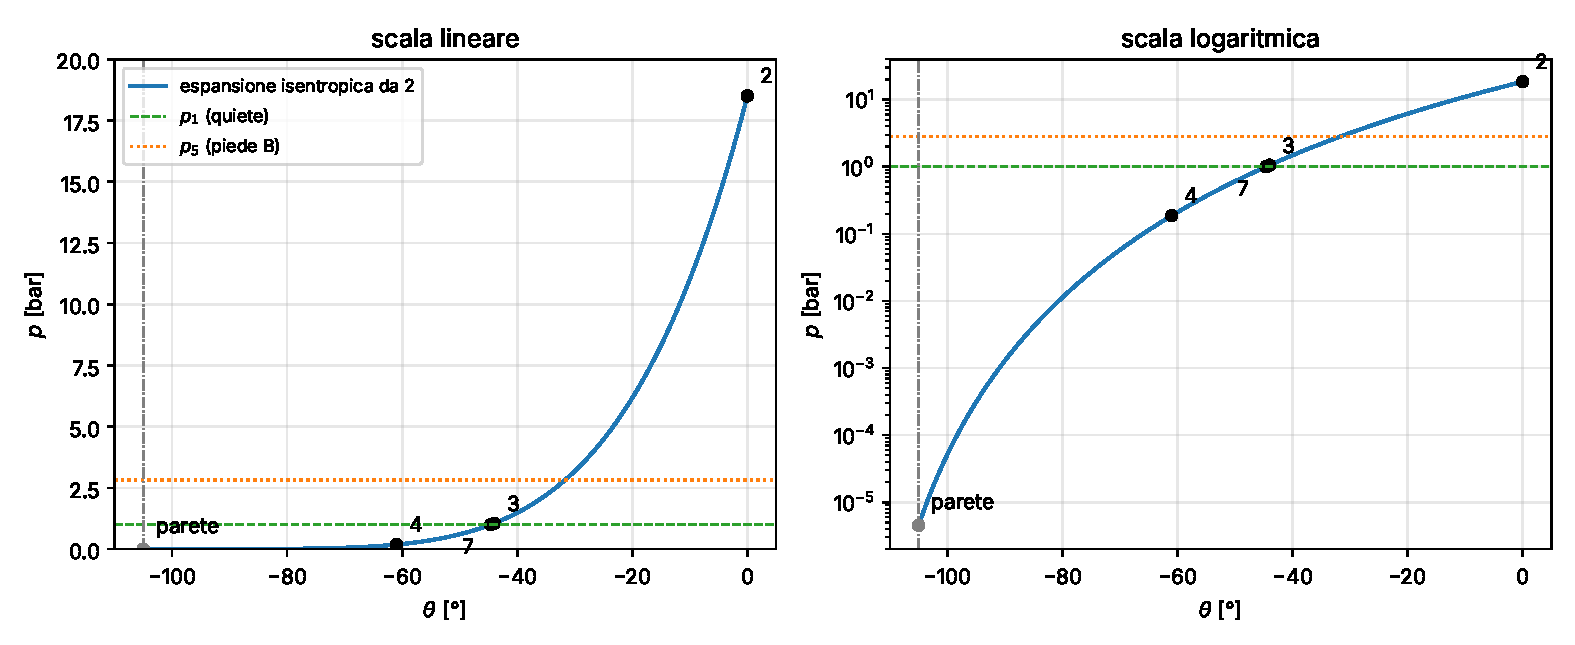
\includegraphics[width=\textwidth]{p_theta.pdf}
  \caption{Piano $p$--$\theta$: curva dell'espansione isentropica dallo stato 2 ($\theta$ decrescente, onde $\Cp$), con
  gli stati 2, 3, 4, lo stato asintotico 7 a $p=p_1$ e il punto ``parete'' che si avrebbe seguendo la rotazione di
  \ang{105}. A sinistra la scala lineare, a destra quella logaritmica.}
  \label{fig:pt}
\end{figure}
Le pressioni vanno da $\SI{18.5e5}{Pa}$ a meno di $\SI{0.2e5}{Pa}$, e fino a pochi pascal per la parete attaccata.
La scala lineare mostra come quasi tutta la caduta di pressione avvenga nei primi 20--30 gradi di rotazione. Oltre
\ang{-45} la curva è schiacciata sull'asse: 3, 4 e 7 sono indistinguibili da $p=0$ rispetto a $p_2$. La scala
logaritmica separa gli stati. Si vede che 3 e 7 coincidono quasi sulla retta $p=p_1$: la deviazione di SL in C è
quella asintotica. Lo stato 4 sta un ordine di grandezza sotto $p_1$ e sotto $p_5$: da qui la necessità di RC. Infine
la parete attaccata ($p\sim10^{-5}$ bar) è di fatto il vuoto. Gli stati 5 e 6 non stanno su questa curva: sono
prodotti da urti mobili, e compaiono come livelli di riferimento.

\begin{figure}[H]
  \centering
  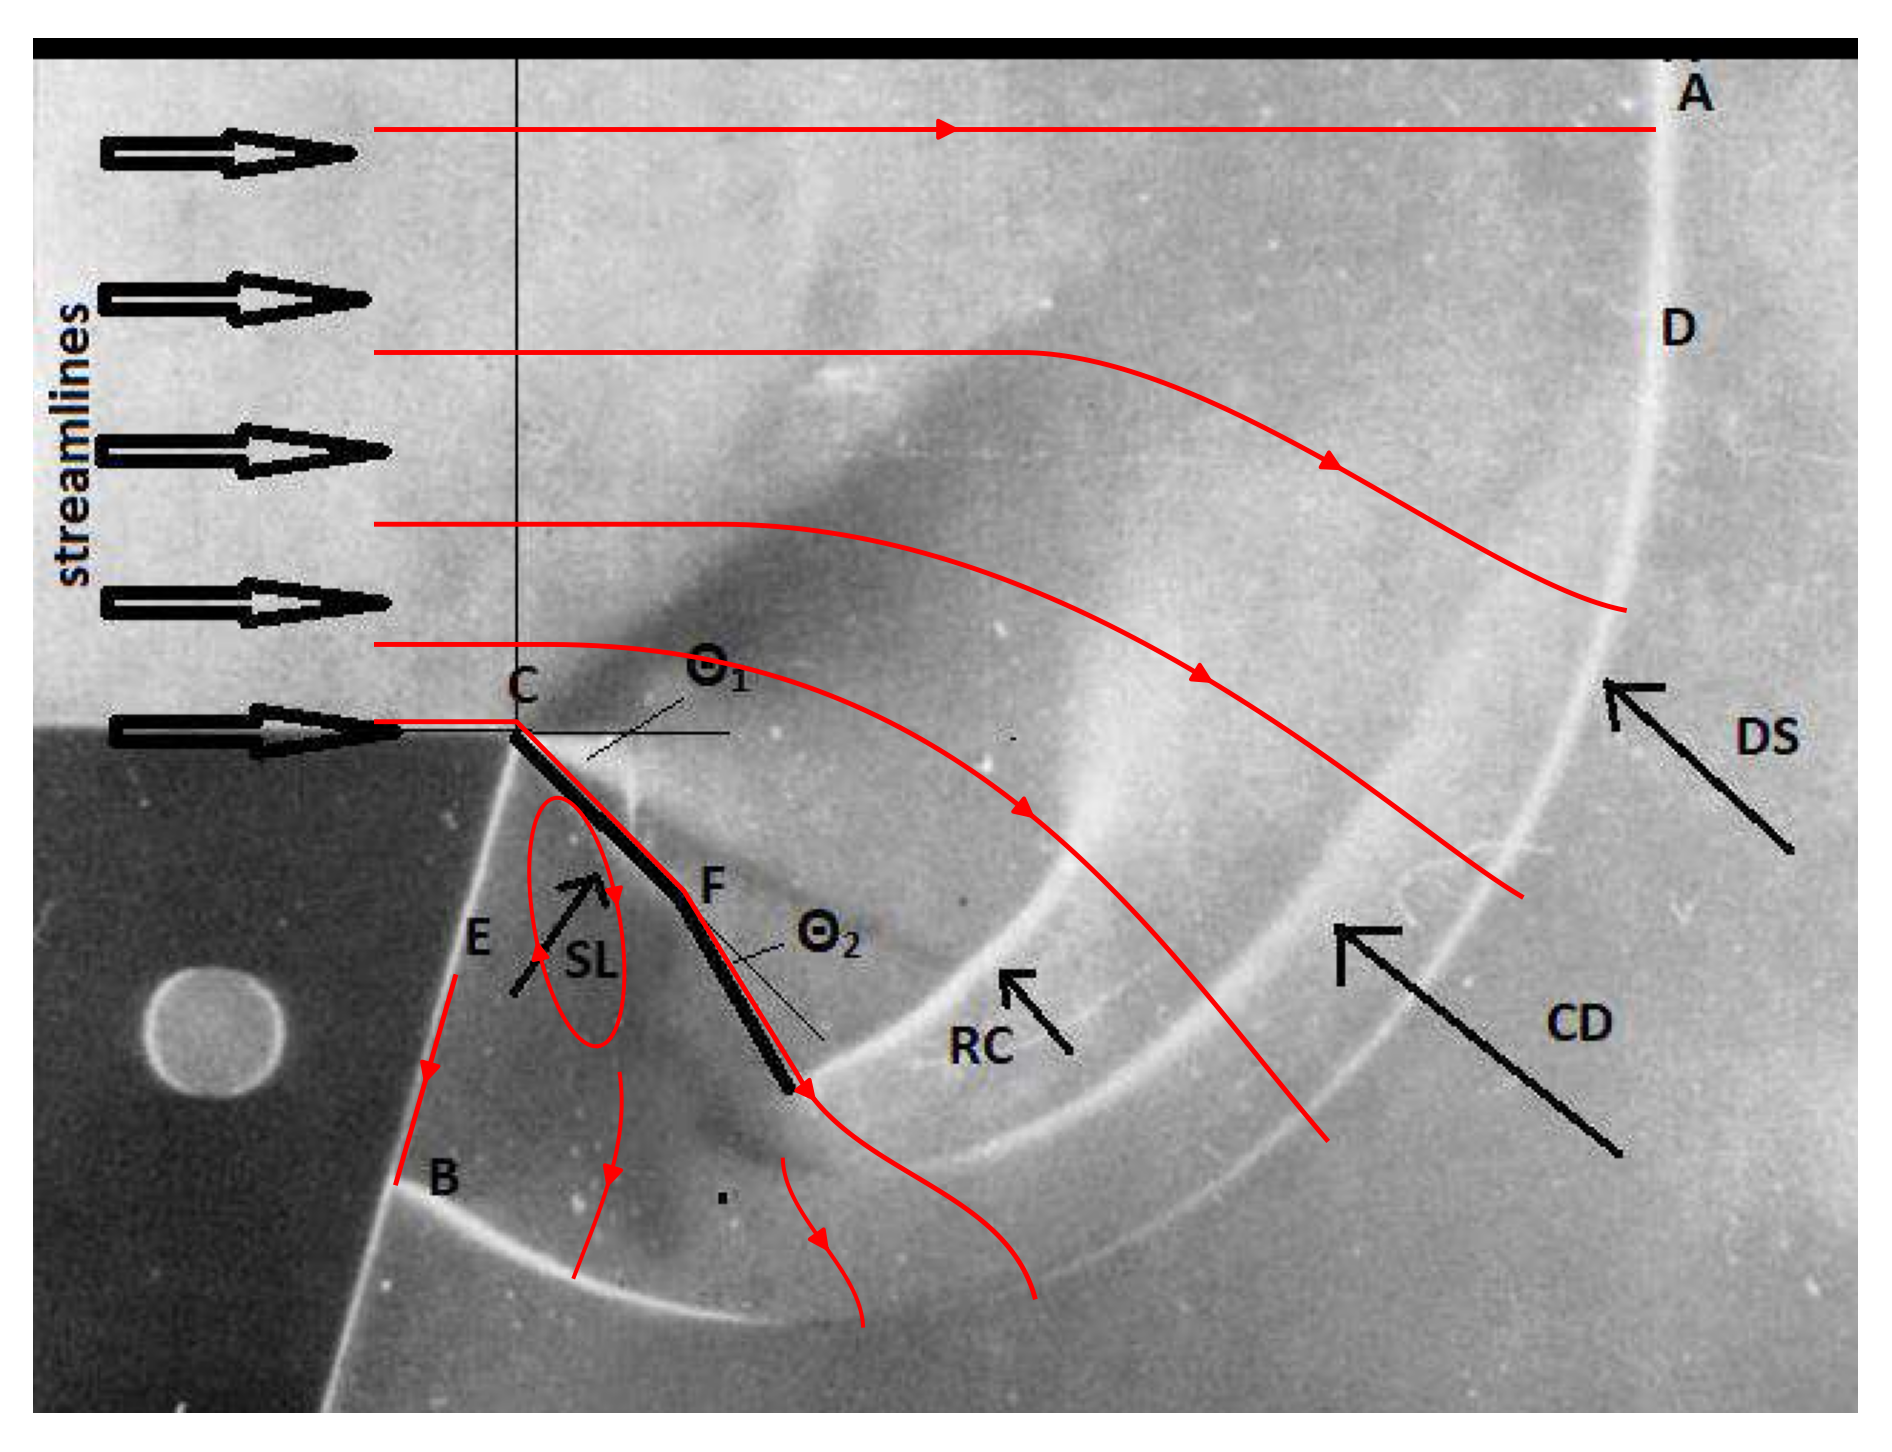
\includegraphics[width=0.86\textwidth]{linee_corrente.png}
  \caption{Linee di corrente all'istante della foto, nel riferimento del laboratorio: orizzontali nello stato 2 sopra
  la testa del ventaglio; deviate nel ventaglio di C, fino a seguire SL e il secondo tratto dopo F; ortogonali a DS
  nel gas che DS mette in moto; ricircolo nella bolla fra CE e SL; scorrimento lungo la parete da E verso B.}
  \label{fig:lc}
\end{figure}
Nella figura delle linee di corrente le linee più alte arrivano all'urto piano senza deviare, perché la testa del
ventaglio non le raggiunge. Le altre ruotano tanto più quanto più passano vicino a C. Dopo RC e CD si raccordano alla
direzione normale a DS: la direzione cambia con continuità da orizzontale (vicino a D) a parallela alla parete
(in B).

%==============================================================================
\section{Coerenza con l'immagine e discussione}
\textbf{Confronti con la foto.}
\begin{itemize}
\item La testa calcolata (retta a $\mu_2=\ang{40}$) coincide con il bordo della zona scura misurato a circa \ang{43}.
\item Il punto D calcolato è a $0{,}45\,x_A$, quello visibile a circa $0{,}35\,x_A$. In D il disturbo che arriva
  all'urto è un'onda acustica, cioè infinitesima: la curvatura di DS parte con pendenza nulla e diventa apprezzabile
  solo più in basso. Il punto in cui l'occhio vede la curva è quindi più basso del vero D.
\item E calcolato a $0{,}51\,\overline{CB}$ concorda con la posizione indicata sulla traccia.
\item RC si vede netto nel tratto inferiore e si sfuma salendo nel ventaglio, come previsto dal raggio a \ang{24}
  oltre il quale non può più esistere.
\end{itemize}

\textbf{Stato 4 e RC sono stime.} Nel ventaglio di F e dietro RC il campo non è uniforme. La pressione bassa del
nucleo del vortice, che piega SL in F, è un effetto viscoso e rotazionale che il modello non descrive: lo prendo dalla
misura di $\theta_2$. RC è curvo e la sua velocità varia lungo il fronte; $W_{RC}\approx W_B$ è una stima geometrica.
Il livello di $p_6$ che ne risulta è comunque coerente con il gas compresso da DS. La ricostruzione completa della
zona fra RC, CD e DS (subsonica rispetto alla configurazione e a due famiglie) richiederebbe la soluzione numerica del
campo pseudo-stazionario. Qui basta sapere che la pressione sale da circa $p_5$ al piede fino a $p_2$ in D.

\textbf{Intensità decrescente dell'urto.} L'urto passa da $\Ms=4$ in D a $1{,}6$ in B: il salto di pressione cala da
18,5 a 2,8. Il gas investito vicino alla parete inclinata riceve circa un ventesimo dell'entropia di quello investito
dall'urto piano ($\Delta s/R=0{,}11$ contro $1{,}98$): è questo il salto che rende visibile CD.

\textbf{Campo asintotico.} Lo spigolo si comporta come il labbro di un getto sottoespanso con $n=p_2/p_1=18{,}5$, con il
contorno isobaro alla pressione ambiente. La deviazione $\theta_{SL,\infty}\approx\ang{44.6}$ coincide con la $\theta_1$
misurata perché l'intorno dello spigolo, in un campo autosimile, è già il campo asintotico.
\end{document}
